\section{eo\-External\-Init$<$ F, External, External\-EO $>$ Class Template Reference}
\label{classeo_external_init}\index{eoExternalInit@{eoExternalInit}}
Initialization of external struct, ctor expects a function of the following signature:.  


{\tt \#include $<$eo\-External\-Op\-Functions.h$>$}

Inheritance diagram for eo\-External\-Init$<$ F, External, External\-EO $>$::\begin{figure}[H]
\begin{center}
\leavevmode
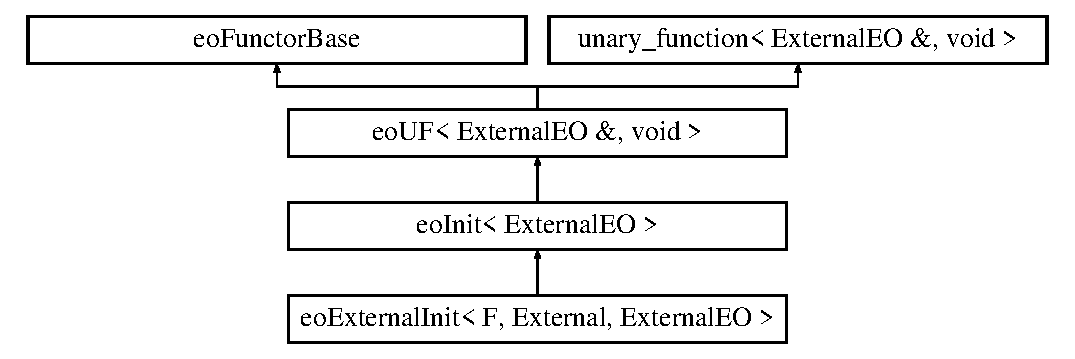
\includegraphics[height=4cm]{classeo_external_init}
\end{center}
\end{figure}
\subsection*{Public Member Functions}
\begin{CompactItemize}
\item 
{\bf eo\-External\-Init} (External($\ast$\_\-init)(void))\label{classeo_external_init_a0}

\item 
void {\bf operator()} (External\-EO \&\_\-eo)\label{classeo_external_init_a1}

\begin{CompactList}\small\item\em The pure virtual function that needs to be implemented by the subclass. \item\end{CompactList}\end{CompactItemize}
\subsection*{Private Attributes}
\begin{CompactItemize}
\item 
External($\ast$ {\bf init} )(void)\label{classeo_external_init_r0}

\end{CompactItemize}


\subsection{Detailed Description}
\subsubsection*{template$<$class F, class External, class External\-EO = eo\-External\-EO$<$F, External$>$$>$ class eo\-External\-Init$<$ F, External, External\-EO $>$}

Initialization of external struct, ctor expects a function of the following signature:. 

External func();

Where External is the user defined struct or class 



Definition at line 45 of file eo\-External\-Op\-Functions.h.

The documentation for this class was generated from the following file:\begin{CompactItemize}
\item 
eo\-External\-Op\-Functions.h\end{CompactItemize}
